\documentclass[11pt, bibliography=totoc]{scrartcl}
\usepackage[ngerman]{babel}
\usepackage[utf8]{inputenc}
\setlength{\parskip}{5.5pt}
\setlength{\parindent}{1em}
\usepackage{hyperref}
\usepackage{mathtools}
\usepackage[numbers]{natbib}
\usepackage{url}
\usepackage{algpseudocode}
\usepackage{algorithm}
\usepackage{listings} 
\usepackage{amssymb}
\usepackage{graphicx}
\usepackage{amsmath}
\usepackage[normalem]{ulem}
\usepackage{soul}
\usepackage{color}
\usepackage[table,xcdraw]{xcolor}
\usepackage{pdflscape}
\usepackage{booktabs}
\usepackage{longtable}
\usepackage{geometry}
\usepackage[T1]{fontenc}% wichtig für Trennung von Wörtern mit Umlauten
\usepackage{microtype}% verbesserter Randausgleich
\usepackage[toc,page]{appendix}
\usepackage[all]{nowidow}
\usepackage[style=base, margin=5mm]{caption}
\usepackage{siunitx}

\geometry{a4paper,left=30mm,right=30mm, top=30mm, bottom=35mm} 

%math packages
\usepackage{amsmath}
\usepackage{amsfonts}
\usepackage{amssymb}

%header
\usepackage{fancyhdr}
\pagestyle{fancy}
\fancyhf{}
\chead{\nouppercase{\leftmark}}
\cfoot{\thepage}

\begin{document}


\title{Methoden zur automatisierten Farbgestaltung von Webseiten aus Bildvorlagen.}
\subtitle{Masterprojekt}
\author{Philipp Anders}

\pagenumbering{gobble} % no page numbering
\maketitle

\begin{abstract}
\end{abstract}

\pagebreak
\tableofcontents
\pagebreak

\pagenumbering{arabic} % start page numbering

\section{Einleitung}

Ziel dieser Arbeit ist die Untersuchung von Methoden zur automatisierten Bestimmung der Farbwerte von Oberflächenelementen in Webseiten, welche sich an einer Bildvorlage orientieren. Die Beantwortung dieser Fragestellung erfolgt durch den Vorschlag und die Umsetzung eines konkreten Verfahrens. \autoref{sec:modellierung} unternimmt eine grundlegende Modellierung des Färbungsproblems in Bezug auf Webseiten und legt  den Rahmen der Zielstellung fest. \autoref{sec:cpe} stellt das Teilproblem der Ermittlung repräsentativer Farben eines Bildes vor. \autoref{sec:literatur} ordnet die Arbeit in den aktuellen Forschungskontext ein.

\subsection{Problemmodellierung}
\label{sec:modellierung}

Der CSS-Standard zur Beschreibung der Formatierung von HTML-Dokumenten definiert mehr als 10 Eigenschaften zur farblichen Gestaltung, wobei einige spezifisch für bestimmte  HTML-Elemente sind  \citep{css3-color}. In dieser Arbeit werden die Farbeigenschaften von zwei verschiedenen Arten von Oberflächenelementen $e = (c_\text{text}, c_\text{background}) = C \times C$ betrachtet:
\begin{enumerate}
	\item \textbf{Textelemente} $e_\text{Text}$: Elemente mit transparentem Hintergrund und definierter Vordergrundfarbe (z.B. \texttt{<h1>}, \texttt{<a>}, etc.). Diese besitzen die CSS-Eigenschaften \{ \texttt{background-color: transparent}, \texttt{color:} $e.c_\text{text}$\}.\\ Dementsprechend gilt: $type(e) = \text{Text} \implies e.c_\text{background} = "\text{transparent}"$.\\
	\item  \textbf{Blockelement} $e_\text{Block}$: Elemente, die visuell als Blöcke wahrgenommen werden (z.B. \texttt{<div>}, \texttt{<button>}, etc.). Diese besitzen die CSS-Eigenschaften \{ \texttt{background-color:} $e.c_\text{background}$, \texttt{color:} $e.c_\text{text}$\}.
\end{enumerate}
Es wird also die Farbbestimmung von Vorder- und Hintergrundfarben fokussiert. Rahmen, Textdekoration und andere färbbare Eigenschaften werden vernachlässigt.

Üblicherweise werden mehrere Elemente eines HTML-Dokuments auf die gleiche Farbe abgebildet. Ein Beispiel ist die Darstellung aller Links ($e.c_\text{text}$) sowie Buttons ($e.c_\text{background}$) in Blau. Im Folgenden wird eine Liste von Elementen einer Webseite mit gleicher Farbabbildung als \textbf{Color Group} $CG = (e_1, e_2, ...) $ bezeichnet \citep[siehe auch][]{webpage, patterns}. Die Menge aller Color Groups einer Webseite heißt \textbf{Color Groups} $CGs = \{CG_1, ... CG_m\}$ mit $|CGs| = m$. Abbildung \ref{fig:colorgroups} veranschaulicht dies anhand einer exemplarischen Webseite für Musik-Streaming. (a) zeigt ein generisches Farbdesign, während (b) die sechs Color Groups separat hervorhebt.

\begin{figure}[]
	\centering
	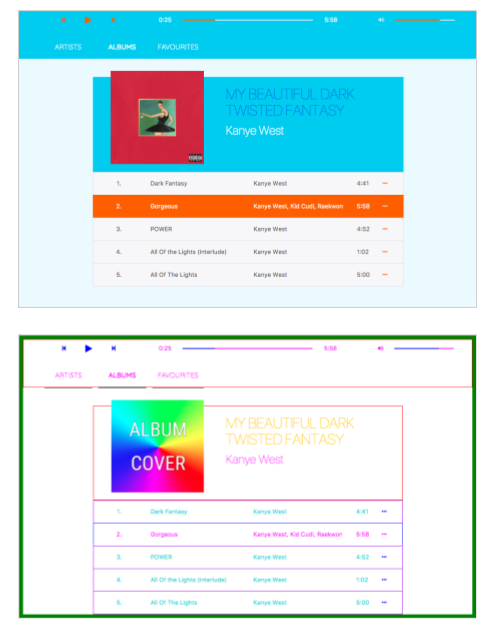
\includegraphics[width=1\textwidth]{img/color_groups.png}
	\caption{Beispiel der Farbgestaltung einer exemplarischen Weboberfläche für Musik-Streaming. (a) Generische Farbgestaltung ohne Anpassung an das Albumcover. (b) Separate Hervorhebung der sechs Color Groups. Elemente einer Color Groups sind jeweils rot dargestellt. (c) Beispiel einer Farbgestaltung mit Anpassung an das Album Cover.}
	\label{fig:colorgroups}
\end{figure}

\textcolor{red}{TODO: Abbildung updaten}

Webdesigner verkleinern den Suchraum zur Identifizierung geeigneter Farben für die Color Groups durch die Verwendung einer sogenannten \textbf{Farbpalette} \citep{webpage, webdesign, webx0}. Dabei handelt es sich um eine Farbmenge $P = \{c_1, c_2, \ldots, c_n\}$ mit $n$ Farben, wobei jedes $c \in P$ als String von RGB Werten kodiert wird. \textbf{Die Farbgestaltung einer Webseite ist die Abbildung $f_\text{coloration}: CGs \to P$} mit folgender Definition:

\begin{equation}
\begin{gathered}
  f_\text{coloration}: CGs \to P,\; \\[-1mm] 
  \mathclap{\rule{4cm}{0.4pt}}\\
  f_\text{coloration}(CG) = c \implies \forall e \in CG:
  	\begin{cases}
		e.c_\text{text} = c, \; \text{wenn } type(e) = \text{Text} \\
		e.c_\text{background} = c, \; \text{wenn } type(e) = \text{Block}
	\end{cases}
\end{gathered}
\end{equation}

Entscheidendes Kriterium für die Zuordnung  ist eine funktionale Gestaltung der Webseite. Im Rahmen dieser Arbeit wird hierunter eine Färbung der Oberflächenelemente verstanden, die \textbf{Textlesbarkeit} und \textbf{Benutzerführung} gewährleistet. Eine intuitiv widersinnige Färbung ist beispielsweise roter Text auf orangem Hintergrund mit grauem Button. Weder ist der Text lesbar, noch wird die Aufmerksamkeit des Nutzers auf das Interaktionselement gelenkt.

Die Farbpalette soll auf einer Bildvorlage basieren. So wird eine Harmonisierung des visuellen Eindrucks einer Weboberfläche und einer darin präsenten Grafik erreicht. Da die Farben einer Webseite wesentlich für deren vermittelte Atmosphäre sind \citep{webdesign}, soll die Anpassung der Farbgebung an ein Motiv den Eindruck des Bildes unterstützen. Da die Farbpalette somit auf den verarbeiteten Daten basiert, ist eine Berechnung der Farbgestaltung einer Webseite zur Laufzeit möglich. Ein Anwendungsbeispiel hierfür ist die farbliche Anpassung einer Webanwendung für Musikstreaming an das gespielte Albumcover. Abbildung \ref{fig:colorgroups} (c) zeigt hierfür ein Beispiel. Die Ermittlung von $P$ aus einer Grafik wird als Color Palette Estimation bezeichnet und im Folgenden besprochen.

\subsection{Color Palette Estimation}
\label{sec:cpe}

Die Abbildung einer Bildvorlage $I$ auf eine Farbpalette $P$ wird von \citet{acopa} als \textbf{Color Palette Estimation} (CPE) $f_{CPE}: I \to P$, bezeichnet und als die Repräsentation eines Bildes mit einer minimalen Menge von Farben beschrieben. \glqq{}Minimal\grqq{} bedeutet nach Auffassung der Autoren, dass redundante Farben reduziert und die seltenen Farben der für die Wahrnehmung wichtigen Objekte erhalten bleiben. Formale Kriterien werden hierfür jedoch nicht geliefert. Abbildung \ref{fig:ladybug} veranschaulicht diese intuitive Definition am Beispiel eines Bildes mit einem Marienkäfer, dessen Sichtbarkeit von der Wahl der Farbpalette abhängt.

\begin{figure}[h]
\centering
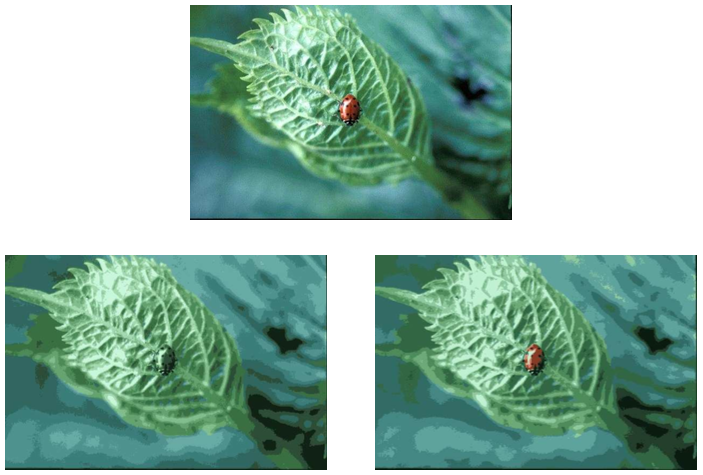
\includegraphics[width=0.5\textwidth]{img/ladybug.png}
\caption{Beispiel für die Einfärbung eines Bildes mit unterschiedlichen Farbpaletten der Größe 12. Oben: Originalbild. Links: Farbpalette ohne rote Farbtöne. Rechts: Farbpalette mit roten Farbtönen, wodurch der Marienkäfer erkennbar ist (Quelle: \citep{acopa})}
\label{fig:ladybug}
\end{figure}

Historisch geht die CPE aus der Farbquantisierung hervor, bei der die Farben von Grafiken aufgrund der damals zu kleinen Kapazität von Grafikpuffern vor deren Anzeige reduziert (Farbreduktion) und dann auf die reduzierte Farbpalette abgebildet wurden (Quantisierung) \citep{variance}. Aus diesem Kontext kommt das formale Kriterium der Summe des quadratischen Fehlers, welcher in diesem Anwendungsfall auch als \emph{Recoloring Error} bezeichnet wird \citep{colorthemes}. Da Grafikpuffer mittlerweile über ausreichend Kapazität verfügen liegt die Anwendung der CPE in anderen Bereichen, wie z.B. der farbbasierten Indizierung von Grafiken in Datenbanken oder der Zusammenstellung von Farbpalletten zu Gestaltungszwecken. \citet{colorthemes} zeigen, dass in letzterem Kontext der Recoloring Error keine geeignete Metrik zur Beurteilung der Güte einer Farbpalette in Bezug auf die Bildvorlage ist. Dies beruht auf den menschlichen Wahrnehmungseigenschaften, wobei Bilder auf Komponenten- und nicht auf Pixelebene erfasst werden. Stattdessen werden eine Reihe anderer Metriken vorgestellt, die diesen Umstand berücksichtigen. Die Autoren zeigen zusätzlich empirisch, dass abhängig vom Individuum ein und dieselbe Farbpalette im Bezug auf die Bildvorlage als unterschiedlich repräsentativ bewertet wird.

Dieser Befund hebt hervor, dass die Güte der Abbildung $I \to P$ subjektiv ist und vom Anwendungsbezug abhängt. Aus diesem Grund wird für die Beurteilung der zu ermittelnden Farbpalette keine objektive Bewertungsfunktion herangezogen. Stattdessen wird die Auswahl eines Algorithmus zur CPE fokussiert, dessen resultierende Farbpalette zweckmäßig in Hinblick auf die farbliche Gestaltung von Webseiten ist. Hierfür werden in \autoref{sec:farbgestaltung} Prinzipien für eine funktionale Gestaltung von Webseiten sowie Farbdefinitionen in Style Guides analysiert.

\subsection{Einordnung und Literaturbesprechung}
\label{sec:literatur}

Diese Arbeit ordnet sich in das Gebiet der automatisierten Farbgestaltung (\emph{Color Design Automation}) ein. In diesem Bereich hat in den letzten Jahren Forschung in verschiedenen Anwendungsbezügen stattgefunden, wobei überwiegend Methoden des maschinellen Lernens zur Problemlösung zum Einsatz kommen.

\citet{colorcomp} haben 2011 ein Regressionmodell zur Bewertung der Farbkompatibilität von bis zu fünf Farben entwickelt, d.h. zur Bewertung der Farbharmonie einer Farbpalette. Hierfür wurde ein Training an den Datenbeständen von Farbpaletten-Communities wie z.B. Adobe Color\footnote{\url{https://color.adobe.com/de/explore/}} durchgeführt. Dabei hat sich unter anderem ergeben, dass die auf geometrischen Strukturen im Farbkreis beruhenden Modelle der klassischen Farbentheorie Farbhamonien nicht zufriedenstellend voraussagen und in bestimmten Fällen sogar kontraproduktiv sind. Hierzu zählen zum Beispiel die Farbton-Schablonen von \citet{itten} oder \citet{munsell}. Die Grenzen des Modells liegen in der Bewertung der Harmonie von Farben mit unterschiedlicher räumlicher Ausprägung \citep{webpage, patterns}. Eine Matlab-Implementierung des Modells zur Überprüfung von Farbharmonien steht öffentlich zum Download bereit\footnote{\url{http://www.dgp.toronto.edu/~donovan/color/}}.

\citet{patterns} haben sich 2013 mit der Lösung einer grundlegenden Form eines Färbungsproblems auseinandergesetzt: Die Kolorierung von Mustern nach dem Prinzip "Malen nach Zahlen". Hierfür wurde ein probabilistisches Modell entwickelt, indem über 8000 von Künstlern entworfene Muster ausgewertet wurden\footnote{\url{http://www.colourlovers.com/}}. Konkrete Färbungslösungen werden durch einen \emph{Factor Graph} ermittelt, was ebenfalls einen Ansatz für die vorliegende Arbeit darstellt. Das Modell von \citet{colorcomp} wird als externer Bestandteil des Graphen hinzugefügt, um eine globale Kompatibilität der eingesetzten Farben zu gewährleisten. Eine Anwendung, welche die Autoren vorschlagen, stellt die Umkehrung des Ziels dieser Arbeit dar: Die Anpassung eines Musters an das Farbschema einer Webseite.

\citet{webpage} haben sich 2016 mit der automatisierten Farbgestaltung von Webseiten auseinandergesetzt. Durch die Auswertung von 500 Webseiten wurde ein probabilistisches Modell in Form eines Optimierungsproblem mit drei Zielfunktionen entwickelt. Zielfunktionen 1 gewährleistet einen ausreichenden Kontrast zwischen den Oberflächenelementen. Zielfunktion 2 passt die Farbgestaltung an ein Schlüsselwort an (z.B. \glqq{}Business\grqq{} oder \glqq{}Fresh\grqq{}). Zielfunktion 3 wird durch das Modell von \citet{colorcomp} realisiert und gewährleistet Farbharmonie. Die Optimierung wird durch eine lexikographische Strategie umgesetzt, bei welcher in Interaktion mit einem Gestalter die Zielfunktionen nacheinander angewendet werden. Die Farben zur Seitenfärbung werden Farbpaletten von Adobe Color\footnote{\url{https://color.adobe.com/de/explore/}} entnommen. Als alternatives Anwendungsbeispiel extrahieren die Autoren eine Farbpalette aus einer Grafik und nutzen diese als Grundlage zur Färbung, was dem Ziel der vorliegenden Arbeit entspricht. Zur CPE wird der K-Means Algorithmus verwendet. Somit ist der vorgestellte Prozess der Autoren im Gegensatz zum Ziel dieser Arbeit lediglich teilautomatisiert. Einerseits muss ein geeignetes $k$ des K-Means Algorithmus vom Anwender ermittelt werden, andererseits erfordert die lexikographischen Strategie bei der Optimierung eine Nutzerinteraktion. Somit handelt es sich bei der Lösung um ein Unterstützungswerkzeug für Webdesigner und nicht um ein System zur vollautomatisierten Farbgestaltung einer Webseite.

\citet{magazines}  haben sich 2013 mit der automatisierten Farbgestaltung von Magazin-Covers auseinandergesetzt. Vergleichbar mit \citep{webpage} wird ebenfalls die Optimierung des Farbkontrasts, der Farbharmonie und der Farbsemantik verfolgt. Im Gegensatz zu den bisherigen Lösungen wird allerdings mit expliziten Regeln zur Bewertung von Farbharmonien- \citep{itten} und Kontrasten anstatt mit Modellen gearbeitet, die sich aus Trainingsdaten ableiten. Über Flowcharts vermitteln die Autoren Lösungsprozeduren zur Suche geeigneter Schriftfarben unter Beachtung des Kontrasts, welche eine Anregung für die vorliegende Arbeit darstellen.

\section{Farbgestaltung von Webseiten}
\label{sec:farbgestaltung}
Die Ziele der farblichen Gestaltung im Rahmen dieser Arbeit sind Lesbarkeit und Benutzerführung. Konkrete Kriterien für die Textlesbarkeit werden in \autoref{sec:lesbarkeit} vorgestellt. In  \autoref{sec:usability} wird der Begriff Benutzerführung erläutert und damit im Zusammenhang stehende Gestaltungsprinzipien im Webdesign herausgearbeitet. Davon ausgehend wird in \autoref{sec:architecture} ein konkreter Vorschlag für eine Systemarchitektur zur automatisierten Farbgestaltung von Webseiten erarbeitet.

\subsection{Lesbarkeit}
\label{sec:lesbarkeit}

\begin{figure}[]
	\centering
	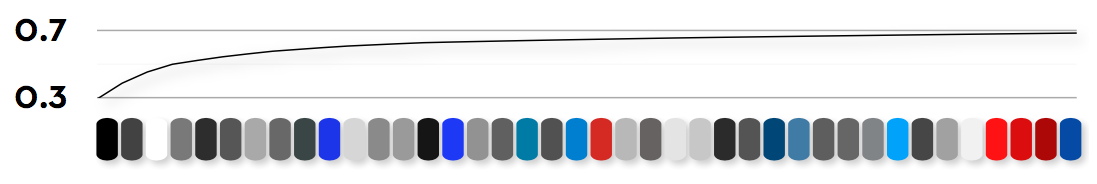
\includegraphics[width=0.7\textwidth]{img/webzeitgeist_textcolors.png}
	\caption{Die 40 populärsten Textfarben in Webseiten machen $70\%$ aller verwendeten Textfarben aus. (Quelle: \citep{webzeitgeist})}
	\label{fig:webzeitgeist_textcolors}
\end{figure}

\autoref{fig:webzeitgeist_textcolors} zeigt, dass gemäß einer Auswertung von über 100.000 Webseiten Text in HTML-Dokumenten fast ausschließlich in Graustufen dargestellt wird \citep{webzeitgeist}. Die populärsten Farben sind Schwarz, Dunkelgrau und Weiß. \citet{webdesign} begründet dies damit, dass Text schlechter lesbar wird, je bunter er ist. Der Style Guide von Googles Material Design \citep{google} hebt hervor, dass Aufgrund des Simultankontrasts die Verwendung von Grau als Textfarbe bei Hintergrund mit hoher Buntheit zu unerwünschten Effekten führt, wie Abbildung \ref{fig:text_color} veranschaulicht. Stattdessen wird in Abhängigkeit von der Helligkeit des Hintergrunds die Verwendung von Schwarz bzw. Weiß mit einem Alpha-Wert (Transparenz) empfohlen. Konkret werden folgende Werte genannt:
\begin{enumerate}
	\item Dunkle Schrift: $\text{rgba}(0, 0, 0, 0.87)$
	\item Helle Schrift: $\text{rgba}(255, 255, 255, 1.0)$
\end{enumerate}

\begin{figure}[h]
	\centering
	
\includegraphics[width=0.95\textwidth]{img/text_color.png}
	\caption{Empfohlene Textfarbe bei buntem Hintergrund. (a) Textfarbe $\text{rgb}(114,114,114)$. Der Text ist aufgrund des Simultankontrasts unangenehmer zu lesen. (b) Textfarbe $\text{rgba}(0, 0, 0, 0.54)$, d.h. Schwarz mit einem Alphawert  von $54\%$. Die Textfarbe ergibt sich zu einer Verschwärzlichung der Hintergrundfarbe und vermeidet so den Simultankontrast. (Quelle: \citep{google})}
	\label{fig:text_color}
\end{figure}

Es ist zu entscheiden, wann die dunkle und wann die helle Textfarbe verwendet wird. Hierfür geben die Web Content Accessibility Guidelines (WCAG) des W3C konkrete Grenzwerte für Kontrastverhältnisse in Abhängigkeit von der Text-, der Hintergrundfarbe sowie der Textgröße an. Die Formel zur Berechnung des Kontrastverhältnisses $L_c$ lautet \citep{wcag-contrast}:

\begin{equation}
	\begin{split}
		L_c(e.c_\text{text}, e.c_\text{background}) = \frac{L(e.c_\text{text}) + 0.05}{L(e.c_\text{background}) + 0.05} \;,\\
		L(e.c_\text{text}) \geq L(e.c_\text{background})
	\end{split}
\end{equation}

mit $L_c \in [1, ... , 22]$, wobei $L_c(rgb(255, 255, 255), rgb(0, 0, 0)) = 22$ und $e.c_\text{text} = e.c_\text{background} \implies L_c(e.c_\text{text}, e.c_\text{background}) = 1$ gilt. Die Berechnungsvorschrift der normalisierten relativen Luminanz $L()$ einer Farbe ist \citep{wcag-rel-luminance} zu entnehmen.

Es gibt zwei verschiedene Grenzwertklassen \citep{wcag}. Die Grenzwertklasse \emph{AA} beschreibt die Minimalanforderung an lesbaren Text:
\begin{equation}
  	AA: L_c(e.c_\text{text}, e.c_\text{background}) \geq
	\begin{cases}
	3.0, \; \text{size}(e) \geq 18\text{pt} \lor \text{size}(e) \geq 14\text{pt} \land \text{weight}(e) = \text{bold}\\
		4.5,  \;  \text{sonst}
	\end{cases}
\end{equation}

Die Klasse \emph{AAA} beschreibt bessere Lesbarkeit durch die Verwendung höherer Grenzwerte:

\begin{equation}
  	AAA: L_c(c_1, c_2) \geq
	\begin{cases}
		4.5, \; \text{size}(e) \geq 18\text{pt} \lor \text{size}(e) \geq 14\text{pt} \land \text{weight}(e) = \text{bold}\\
		7.0,  \;  \text{sonst}
	\end{cases}
\end{equation}

\subsection{Benutzerführung}
\label{sec:usability}
Ein adäquater Farbeinsatz ermöglicht die Steuerung von Aufmerksamkeit und unterstützt die Bildung von Zusammenhängen \citep{webdesign}.  Dieses Konzept wird auch als visuelle Hierarchy bezeichnet \citep{visual-hierarchy}, bei welchem die Oberflächenelemente bei der Wahrnehmung strukturiert und priorisiert werden.
\citet{webdesign} unterteilt folgende Möglichkeiten zur Benutzerführung durch Farbeinsatz:

\begin{itemize}
	\item \textbf{Themengruppen:} Bedeutet die farbliche Kodierung inhaltlich definierter Bereiche. Hierbei handelt es sich um eine vom Gestalter erfundene, subjektive Farbsystemlogik. Sie stellt kein System, sondern eine Gestaltungsstuktur dar, die dem Anwender zu lernen aufgezwungen wird. Dies resultiert automatisch in Buntheit, welche Aufmerksamkeit erregt und somit kontraproduktiv für die Bildung einer visuellen Hierarchie ist. Aus diesen Gründen ist von dieser Variante abzuraten. Abbildung \ref{fig:theme_coding} verdeutlicht dies am Beispiel eines Online-Magazins.
	\item \textbf{Funktionsbereiche:} Bedeutet die farbliche Abgrenzung von Bereichen mit einheitlicher Funktion. Dies beinhaltet beispielsweise die farbliche Differenzierung von Navigations-, Inhalts- und Servicebereichen. Diese Variante ist zu empfehlen, wenn nicht mehr als drei Farben verwendet werden und die betreffenden Bereiche gleichzeitig und somit im Bezug zueinander sichtbar sind. Abbildung \ref{fig:functional_areas} verdeutlicht dies am Beispiel der farblichen Abgrenzung verschiedener Navigationsbereiche.
	\item \textbf{Funktionen und Zustände:} Bedeutet die farbliche Kodierung verschiedener Elemente mit einheitlicher Funktion. Beispielsweise sind alle anklickbaren Elemente (z.B. Links und Buttons) einer Seite durch eine einheitliche Farbe signalisierbar. Abbildung \ref{fig:functions} zeigt hierfür ein Beispiel. Bestimme Wirkungen können zusätzlich farblich hervorgehoben werden, wie z.B. die rote Färbung von Buttons zum Löschen oder Abbrechen einer Aktion. Wurde eine Farbe einmal mit einer Funktion belegt, soll sie einheitlich verwendet werden. Beispielsweise würde ein nicht-anklickbares, blaues Element in der Oberfläche aus Abbildung \ref{fig:functions} den Nutzer verwirren.
\end{itemize}

\begin{figure}[]
	\centering
	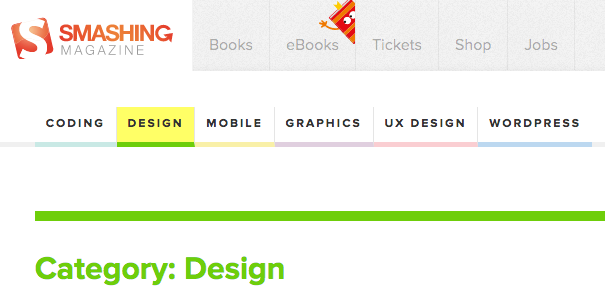
\includegraphics[width=0.48\textwidth]{img/theme_coding.png}
	\caption{Farbkodierung von Themengruppen am Beispiel von \url{www.smashingmagazine.com/}. Es ist unklar, weshalb die gewählten Farben mit den jeweiligen Bereichen assoziiert werden.}
	\label{fig:theme_coding}
\end{figure}

\begin{figure}[]
	\centering
	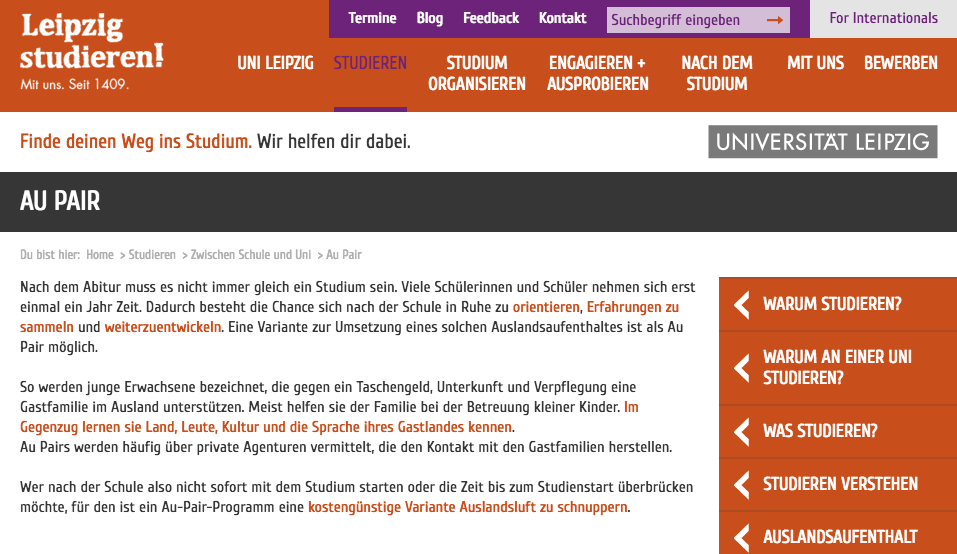
\includegraphics[width=0.48\textwidth]{img/functional_areas.png}
	\caption{Farbkodierung von Funktionsbereichen am Beispiel von \url{www.leipzig-studieren.de}. Navigationsbereiche (orange) werden zueinander in Bezug gebracht und vom Inhalt (weiß) abgegrenzt.}
	\label{fig:functional_areas}
\end{figure}

\begin{figure}[]
	\centering
	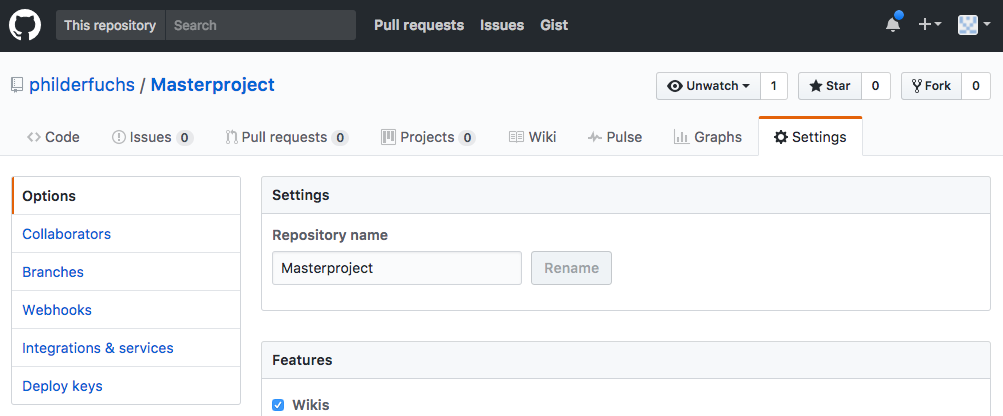
\includegraphics[width=0.48\textwidth]{img/functions.png}
	\caption{Farbkodierung von Funktionen am Beispiel von \url{www.github.com}. Nur anklickbare Elemente sind blau, aktive Elemente werden zusätzlich braun markiert.}
	\label{fig:functions}
\end{figure}

\subsection{Funktionsfarben}
\label{sec:funktionsfarben}

Aus \autoref{sec:usability} geht hervor, dass Farbeinsatz im Webdesign der Abgrenzung von Funktionsbereichen sowie der Kennzeichnung von Elementen mit einheitlicher Funktion dient. Aus diesen Gründen wird die Abbildung $f_\text{coloration}: CGs \to P$ durch eine Abstraktionsschicht erweitert, welche beschreibt, welche Funktion eine Color Group in einer Oberfläche erfüllt. In Anlehnung an \citep{google,  smashing} wird exemplarisch die Menge der Funktionsfarben $F = \{\text{Primär}, \text{Sekundär}, \text{Akzent}, \text{Interaktion}, \text{Text (neutral)}, , \text{Hintergrund (neutral)}\}$ definiert. Deren Bedeutungen lauten wie folgt:

\begin{itemize}
	\item \textbf{Primärfarbe:} Wird in Relation zu den anderen Farben am häufigsten eingesetzt und bildet so die farbliche Grundstimmung der Oberfläche \citep{awwwards}.
	\item \textbf{Sekundärfarbe:} Unterstützt die Farbstimmung der Primärfarbe und orientiert sich dementsprechend an deren Farbton. Durch die Wahl einer Farbe mit geringerer Buntheit tritt sie in der visuellen Hierarchie stärker in den Hintergrund \citep{visual-hierarchy} und unterstützt durch den Qualitätskontrast die Wirkung der Primärfarbe \citep{webdesign}.
	\item \textbf{Interaktionsfarbe:} Signalisiert Elemente, mit denen eine Interaktion möglich ist, z.B. durch klicken. Dies trifft nicht zwangsläufig auf Elemente zu, bei denen der Nutzer ohnehin eine Interaktionsmöglichkeit aufgrund ihrer Funktionsgruppe bereits erwartet, wie z.B. in der Seitennavigation.
	\item \textbf{Akzent:} Signalisiert Elemente mit hoher Priorität in der visuellen Hierarchie. Dies wird durch den sparsamen Einsatz (Quantitätskontrast, \citep{webdesign}) einer Farbe mit hoher Buntheit \citep{visual-hierarchy} erreicht.
	\item \textbf{Text (neutral):} Farbe für Fließtext. Entsprechend \autoref{sec:lesbarkeit} wird hierfür in Abhängigkeit vom Hintergrund Weiß $rgba(255, 255, 255, 1.0)$ bzw. Schwarz $rgba(0, 0, 0, 0.87)$ mit Alpha-Kanal festgelegt.
	\item \textbf{Hintergrund (neutral):} Standardfarbe von Blöcken, die keiner der obigen Farbfunktionen entsprechen. Dies betrifft vorwiegend Blöcke mit Fließtext, so dass Textlesbarkeit zu beachten ist. Dementsprechend sind Graustufen zu bevorzugen \citep{webx0}, wobei entsprechend \autoref{sec:lesbarkeit} ein ausreichender Luminanzkontrast zur Textfarbe zu gewährleisten ist. Darum wird die neutrale Hintergrundfarbe analog zur Textfarbe auf Weiß bzw. Schwarz festgelegt.
\end{itemize}

Die hier verwendeten Funktionsfarben sind exemplarisch. Abhängig von den individuellen Ansprüchen einer Webseite ist die Definition anderer Farbfunktionen denkbar. Bei mobilen Anwendungen ist beispielsweise eine farbliche Differenzierung verschiedener Interaktionsformen sinnvoll (z.B. drücken und wischen).

\subsection{Farbschemata}
\label{sec:farbschemata}

Die Abbildung zwischen den Funktionsfarben $F = \{\text{Primär}, ...\}$ und den tatsächlichen Farben einer Farbpalette $P = \{c_1, ...\}$ wird als die Funktion $f_\text{scheme}: F \to P$ definiert und im Folgenden als \textbf{Farbschema} bezeichnet. Die Farbgestaltung einer Webseite ist damit die Abbildung eines Farbschemas auf eine Farbpalette $f_\text{coloration}: (CGs \to F) \to P$.

Diese Definition eines Farbschemas unterscheidet sich von der Verwendung des Begriffs in der Literatur \citep{webdesign}. In dieser bezeichnet ein Farbschema die Charakteristik einer Farbpalette. Es beschreibt, \emph{wie viele} unterschiedliche Farbtöne eine Farbpalette enthält und in welcher \emph{geometrischen Beziehung} diese zueinander im Farbkreis stehen. Beispielsweise bezeichnet ein \emph{triadisches} Farbschema eine Farbpalette mit drei Farbtönen, die sich in einem Abstand von $120^{\circ}$ zueinander befinden. Genauer wird in  \emph{monochromatische}, \emph{komplementäre (duale)}, \emph{triadische} und \emph{tetraedische} Farbschemen unterschieden, welche Farbpaletten mit einem, zwei, drei oder vier verschiedenen Farbtönen repräsentieren. \citep{underestimated, smashing, google} empfehlen jedoch die Beschränkung auf höchstens 3 Farben im Webdesign, während Graustufen für die Darstellung von Text und Hintergründen dominieren.
    
Dementsprechend werden die Begriffe \textbf{monochrom}, \textbf{dual} und \textbf{triadisch} als Charakterisierung der Funktion $f_\text{coloration}$ in dieser Arbeit adaptiert. \autoref{fig:colorschemes} zeigt hierfür Beispiele. Es wird eine exemplarische Farbpalette abgebildet. Die dargestellten Funktionsfarben entsprechen der in \autoref{sec:funktionsfarben} definierte Menge $F$. Es ist zu erkennen, dass die Textfarben sowie die Hintergrundfarbe bereits unabhängig von der Farbpalette vorgegeben werden. Damit realisiert jedes Farbschema im Rahmen dieser Arbeit einen \textbf{Bunt-Unbunt-Kontrast}, was nach \citep{webx0} eine allgemeine Empfehlung für das Screendesign darstellt. Die Grafik zeigt weiterhin mögliche Abbildungen zwischen den Farbfunktionen und der Farbpalette unter \glqq{}konkrete Farbschemata\grqq{}. Für die neutrale Textfarbe stehen in Abhängigkeit vom jeweiligen Hintergrund im HTML-Dokument Weiß bzw. Schwarz zur Verfügung. Standardmäßig wird Weiß für den neutralen Hintergrund angenommen. Die \emph{dark}-Variante eines Farbschemas veranschaulicht eine Variante mit allgemein dunkler Farbstimmung durch die Verwendung eines dunklen Hintergrundes. Ein monochromes Farbschema beschränkt sich auf einen Farbton in verschiedenen Schattierungen. Dadurch wird ein \textbf{Qualitätskontrast} gebildet, welcher die Wirkung der Farbe mit der größten Buntheit erhöht. Das duale Farbschema besitzt zwei Farbtöne. Da Interaktions- und Akzentfarben weniger häufig auftauchen als die Elemente der Primär- und Sekundärfarben wird hierdurch ein \textbf{Quantitätskontrast} gebildet, der die selteneren Farben zusätzlich betont und so zur Bildung einer visuellen Hierarchie beiträgt. Das exemplarische tertiäre Farbschema bildet die Akzent- und Interaktionsgruppen auf unterschiedliche Farben ab und differenziert diese so zusätzlich. 

\begin{figure}[h]
	\centering
	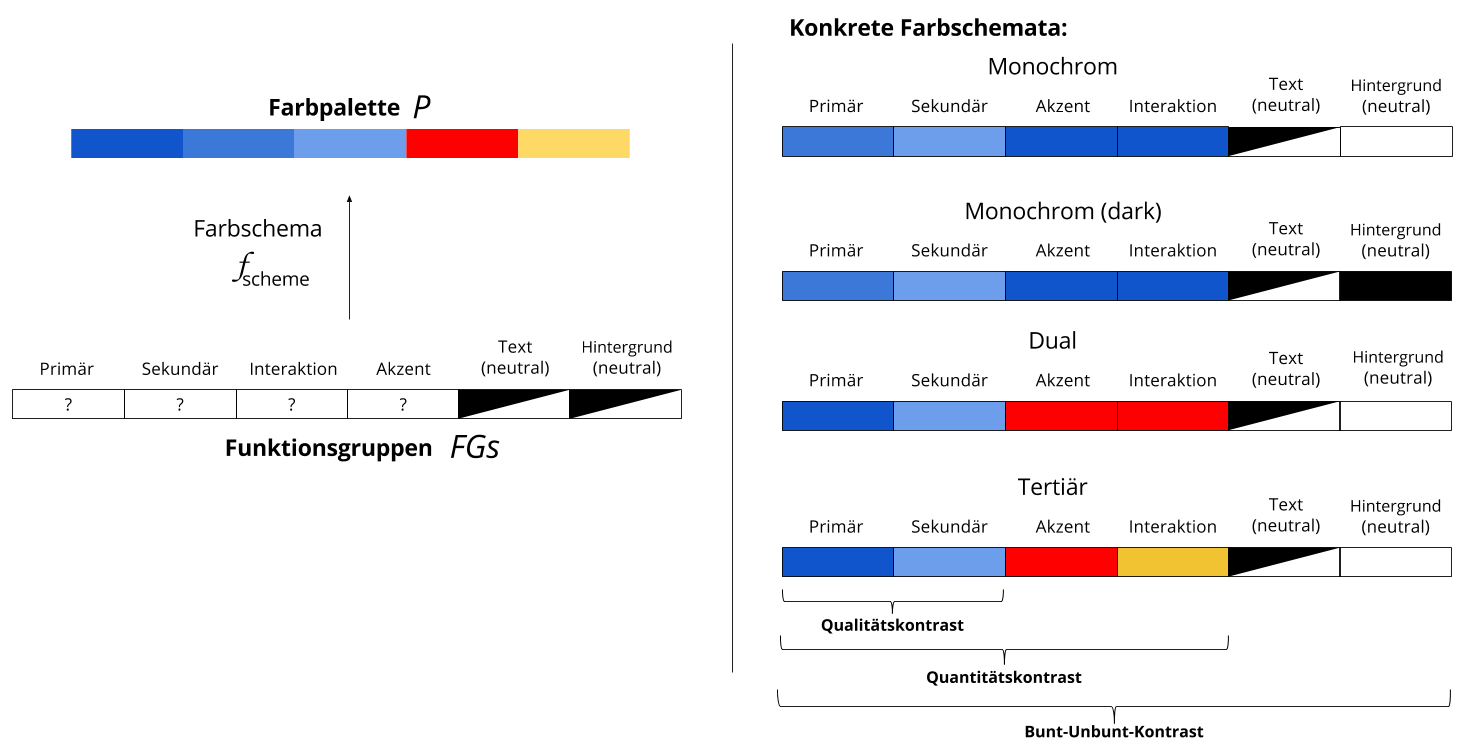
\includegraphics[width=1\textwidth]{img/colorschemes.png}
	\caption{Beispiele für monochrome, duale und tertiäre Farbschemata. Der Farbeindruck der Seite wird durch Quantitäts-, Qualitäts- und Bunt-Unbunt-Kontraste bestimmt.}
	\label{fig:colorschemes}
\end{figure}

\section{Problemlösungsverfahren und Systemarchitektur}
\label{sec:architecture}

Ausgehend von der Literaturbesprechung in \autoref{sec:literatur} sowie den Schlussfolgerungen zur Farbgestaltung von Webseiten in \autoref{sec:farbgestaltung} wird im Folgenden eine Methode zur Problemlösung besprochen. Darauf aufbauend wird in \autoref{sec:architektur} die konkrete Architektur des zu implementierenden Systems vorgestellt.

\subsection{Regelbasierter oder probabilistischer Ansatz}
\label{sec:ansatz}

\citet{webpage} stellen für die automatisierte Farbgestaltung zwei grundlegende Herangehensweisen vor:

\begin{enumerate}
	\item \textbf{Regelbasiert:} Beschreibt quantitative Modelle mit determinstischem Regelwerk. Die Arbeit von \citet{magazines} zur automatisierten Färbung von Magazincovern stellt hierfür ein Beispiel dar. Durch die Analyse von Farbharmonie-Modellen wurden Regeln für Farbbeziehungen abgeleitet.
	\item \textbf{Datengetrieben:} Beschreibt Modelle, welche die Performanz möglicher Lösungen einer automatisierten Farbgestaltung auf Grundlage existierender Beispieldaten vorhersagt.
\end{enumerate}

Die regelbasierten Modelle treffen strickte Aussagen auf einem gewissen Abstraktionsgrad durch eine Vereinfachung des Problems bis zu einer Ebene, auf der Entscheidungen auf Grundlage weniger Parameter getroffen werden (z.B. durch die Angabe fester Grenzwerte). Im Gegensatz dazu stützen sich die Modelle des datengetriebenen Ansatzes auf reale Beispiele und tendieren daher zu robusteren Ergebnissen in der Anwendungsdomäne \citep{webpage}. Durch die Vielfalt der Beispieldaten findet ein verstärkter Einsatz probabilistischer Modelle statt \citep[siehe z.B.][]{webpage, patterns}.

Da bei probabilistischen Modellen alle potentiellen Lösungen bewertet und gegeneinander abgewogen werden müssen, sind hohe Laufzeiten möglich. Die bereits entwickelte Lösung von \citet{webpage} zur automatisierten Farbgestaltung von Webseiten benötigt selbst nach einer Optimierung des Suchverfahrens, bei der unwahrscheinliche Lösungen frühzeitig ausgeschlossen werden, bis zu 2 Stunden zur Konvergenz. Darüber hinaus ist deren vorgestellter Prozess zur Anpassung der Farbgestaltung einer Webseite an eine Bildvorlage nicht im eigentlichen Sinne automatisiert: Einerseits erfordert die Verwendung des K-Means Algorithmus zur CPE die Eingabe der Farbanzahl ($k$) vom Gestalter, andererseits erfordert die lexikographische Strategie einen Nutzerinteraktion während des Optimierungsprozesses.

Aus diesen Gründen wird sich in dieser Arbeit für eine vollautomatisierte, regelbasierte Lösungsmethode entschieden. Auch ohne die Auswertung großer Datenmengen existieren quantitative Modelle zur Gewährleistung der Textlesbarkeit und Benutzerführung, wie z.B. die in \ref{sec:lesbarkeit} vorgestellten quantitativen Grenzwerte der \emph{Web Content Accessibility Guidelines}.

\subsection{Layouts}
\label{sec:layouts}

Ziel dieser Arbeit die Färbung eines konkreten Webseite. Das Parsing eines solchen HTML-Dokuments zur Erschließung aller $e \in CG$ sowie die Speicherung aller topologischen Informationen dieser Elemente innerhalb einer Seite führt jedoch eine zusätzliche Ebene der Komplexität in das zu lösende Problem ein. Der CSS-Standard sieht durch die Klassen-Selektoren \citep{css3-selectors} ohnehin die Auszeichnung einheitlicher darzustellender Elemente bereits auf Ebene der Dokumentenbeschreibung vor. Dementsprechend wird von der konkreten HTML-Beschreibung einer Webseite als  \textbf{Layout} abstrahiert. Ein Layout definiert:

\begin{enumerate}
	\item $FGs$: Die Menge der $k$ Funktionsgruppen $FGs$. Entsprechend \autoref{sec:farbgestaltung} wird diese standardmäßig auf $FGs = \{\text{Primär}, \text{Sekundär}, \text{Akzent}, \text{Interaktion}, \text{Text (neutral)}, \text{Hintergrund (neutral)}\}$ festgelegt.
	\item $CGs$: Die Menge der Color Groups mit den enthaltenen Elementen $CGs = \{CG_1 = (e_1, e_2, ...), ..., CG_m = (e_1, e_2, ...)\}$.
 	\item $CGs \to FGs$: Die Abbildung der Color Groups auf Funktionsgruppen. Beispielsweise definiert ein Layout selbst, welche Elementen interaktiv sind und somit zur Farbfunktion \emph{Interaktion} gehören.
\end{enumerate}

Somit wird die Komplexität der Suchverfahren reduziert, indem die Menge der Funktionsgruppen als konstant angesehen wird und die konkrete Topologie der Oberflächenelemente innerhalb des HTML-Dokuments im Verantwortungsbereich des Layouts liegt.

\subsection{Aufteilung der Suchverfahren}
\label{sec:aufteilung}

Formale stellt sich die automatisierte Farbgestaltung einer Webseite aus einer Bildvorlage als die Abbildung $f_\text{coloration}: (CPs \to FGs) \to (I \to P)$ dar. In \autoref{sec:layouts} wurde dargestellt, dass zur Lösungssuche die Ermittlung der Abbildung $CGs \to FGs$ als gegeben durch das Layout angesehen und somit aus der Betrachtung entfernt wird. Weiterhin existieren die Teilprobleme (1) $f_{CPE}: I \to P$, d.h. die Ermittlung von $n$ repräsentativen Farben einer Bildvorlage sowie (2) Die Ermittlung des Farbschemas $f_\text{scheme}: FGs \to P$, d.h. die Auswahl von $k$ Farben aus der Palette und deren Zuordnung zu den Funktionsgruppen.

In \autoref{sec:architektur} wurde ein regelbasierter Ansatz zur Lösungssuche gewählt. Die Regeln werden im Folgenden als \textbf{Constraints} bezeichnet. Es existieren zwei Herangehensweisen:
\begin{enumerate}
    \item \textbf{Constraints-First}: Setze $|FGs| = k = n = |P|$. $P$ wird in Abhängigkeit vom Layout ermittelt. Hierbei wird die Ermittlung des Farbschemas zum Zeitpunkt der CPE verlagert. Unter Kenntnis der Funktionsgruppen mit deren gewünschten Eigenschaften ist der Suchraum das Histogram der Bildvorlage. Dieser Ansatz wird unter anderem von \citet{colorcomp} verfolgt. Sie verwenden ihr Regressionsmodell zur Bewertung der Farbharmonie, um eine alternative Optimierungsfunktionen zur Suche von $P$ im Farbraum einer Bildvorlage zu formulieren.
    \item \textbf{Constraints-Last}: Setze $k \leq n$. $P$ wird unabhängig vom Layout ermittelt. Der Suchraum für das Farbschema beschränkt sich auf die Farben in $P$. Dieser Ansatz wird ebenfalls von \citep{webpage} bei der datengetriebenen Färbung von Webseiten verfolgt.
\end{enumerate}

Für diese Arbeit wird die Herangehensweise \textbf{Constraints-Last} bevorzugt, um Flexibilität in Bezug auf unterschiedliche Layouts zu gewährleisten. Für die Arbeit bedeutet dies, dass eine Problemlösung anhand eines exemplarischen Layouts mit einer definierten Menge an Funktionsgruppen veranschaulicht wird, eine Übertragung auf andere Layouts jedoch möglich ist.

Selbst unter den gegebenen Einschränkung des Suchraums durch die vorgeschaltete Ermittlung einer Farbpalette ist die Menge potentieller Lösungen mit $\binom{n}{k} k!$ nach wie vor groß. Als Beispiel sei ein Layout mit 5 Funktionsgruppen sowie eine Farbpalette mit 10 Farben gegeben. Somit gilt $|FGs| = k = 5$ und $|P| = n = 10$, wodurch sich $\binom{10}{5} 5! = 30.240$ mögliche Kombinationen ergeben. Dementsprechend ist ein effektives Suchverfahren für die Ermittlung des Farbschemas zu ermitteln. Die von \citet{patterns} verwendeten Factor Graphs stellen hierfür einen Ansatz dar.

\subsection{Systemarchitektur}
\label{sec:architektur}

\begin{figure}
	\centering
	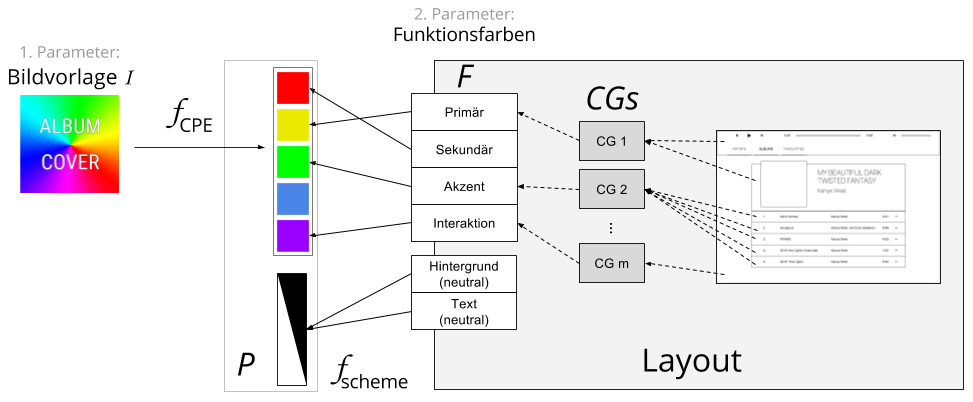
\includegraphics[width=1\textwidth]{img/architecture.png}
	\caption{System-Architektur. Der grau unterlegte Kasten visualisiert den Bereich, für den algorithmische Lösungen gefunden werden müssen. Die Eingabeparameter sind eine Bildvorlage und eine Menge von Color Groups, welche von einem Layout definiert werden. Das System setzt zwei Suchverfahren um, welche mit $f1$ und $f2$ bezeichnet werden. $f1$ ermittelt zuerst eine Farbpalette aus der Bildvorlage (CPE). $f2$ ordnet Colour Groups Farben aus der Palette, in dem ein entsprechendes Constraint System gelöst wird. Nachdem eine Farbabbildung gefunden wurde, wird das kolorierte Layout ausgegeben.}
	\label{fig:architecture}
\end{figure}

Abbildung \ref{fig:architecture} fasst die Systemarchitektur für die die automatisierte Farbgestaltung einer Webseite zusammen. Parameter 1 ist die Bildvorlage \emph{I}, welche durch einen Algorithmus zur Color Palette Estimation $f_{CPE}$ auf eine Menge repräsentativer Farben abgebildet wird. Aus \autoref{sec:usability} folgt, dass unabhängig von der Bildvorlage $weiss$ und $schwarz$ für den neutralen Text bzw. Hintergrund benötigt werden. Darum wird die Farbpalette entsprechend ergänzt: $P_\text{neutral} = f_{CPE}(I) \cup \{weiss, schwarz\}$.

Parameter 2 sind die Funktionsgruppen, welche in \autoref{sec:funktionsgruppen} festgelegt wurden. Durch ein Suchverfahren $f_\text{scheme}$ werden Farben für $\forall fg \in FGs$ gesucht, d.h. es wird ein Farbschema gebildet. Hierfür wird ein Constraint System modelliert, welches durch die von \citet{patterns} vorgestellten Factor Graphs realisiert wird.

Durch die Funktionsgruppen wird im Constraint System von der konkreten Topologie der Oberflächenelemente innerhalb der Webseite abstrahiert. Dies spiegelt sich darin wieder, dass für die Funktionsgruppe \glqq{}Text (neutral)\grqq{} keine bestimmte Farbe durch das Constraint System festgelegt wird, sondern sowohl $weiss$ als auch $schwarz$ zur Auswahl gestellt werden. Darum wird auf der Layout-Ebene für Block-Elemente pauschal diejenige Textfarbe festgelegt, welche unter Verwendung der Formel zur Berechnung des Konstrastverhältnisses $L_c$ aus \autoref{sec:lesbarkeit} den besseren Kontrast liefert:


\begin{equation}
\begin{gathered}
	    \forall FG \in FGs:\\
	    f_\text{scheme}(FG) = c \implies \forall e \in CG \to FG:
  	\begin{cases}
		e = (c, transparent),\; \text{wenn } type(e) = \text{Text} \\
		e = (f_\text{textcolor}(c), c), \; \text{wenn } type(e) = \text{Block}
	\end{cases}\\
	  \mathclap{\rule{4cm}{0.4pt}}\\
 	f_\text{textcolor}: c \to c, f(c) =
  		   	\begin{cases}
  		   		schwarz,\; \text{wenn } L_c(schwarz, c) \geq L_c(weiss, c) \\
		weiss,\; \text{sonst} \\
	\end{cases}
\end{gathered}
\end{equation}

Im Folgenden wird...
\textcolor{red}{Vorschau auf die nächsten Kapitel}

  




\section{Color Palette Estimation}
\label{sec:cpe}

Im Folgenden wird eine Algorithmus zur Lösung des Teilproblems der Ermittlung der Farbobermenge $C_s$ gesucht. Hierzu findet eine Betrachtung von Typen vorhandener Algorithmen zur CPE statt. Abschließend wird ein geeigneter Algorithmus ausgewählt

\subsection{Überblick}

Grundlegend sind zwei Ansätze zur CPE zu unterscheiden:
\begin{enumerate}
    \item \textbf{Hisgoram-basiert}: Algorithmen, die nur auf dem Histogramm des Bildes arbeiten und somit die Positionsinformationen der Farben nicht beachten. Es handelt sich (bis auf Ausnahmen) um Clustering-Verfahren, die durch eine Partitionierung des Farbraums Gruppen ähnlicher Farben im Histogramm identifizieren.
    \item \textbf{Bildsegmentierungs-basiert}: Algorithmen, die durch eine Segmentierung des Bildes zunächst zusammenhängende Komponenten identifizieren und für diese dann repräsentative Farben identifizieren.
\end{enumerate}


Bildsegmentierungs-basierte Algorithmen berücksichtigen die menschlichen Wahrnehmungseigenschaften auf Komponentenebene, führen aber durch die zusätzliche Betrachtung der Positionsinformation eine weitere Komplexitätsebene ein \citep{colorthemes}.

\citet{categorization} treffen eine Kategorisierung der Histogramm-basierten Verfahren in \emph{hierarchisch} und \emph{iterativ}. Hierarchisch arbeitende Algorithmen zur CPE werden auch als \emph{Pre-Clustering Verfahren} bezeichnet, da sie vor dem Erreichen der (fest zu wählenden) Farbanzahl $n$ mit mehr bzw. weniger Farben starten. Sie basieren auf der statistischen Analyse der Verteilung der Bildfarben im Farbraum. In diese Kategorie fallen \emph{top-down} bzw. \emph{bottom-up} Clustering-Algorithmen. Zu den Top-Down Verfahren zählen die in der Vergangenheit populären Raumunterteilungs-Algorithmen wie z.B. Mediancut \citep{mediancut} oder Octree\citep{octree}. Sie Zerteilen den Farbraum sukzessiv in disjunkte Teilräume und unterstellen den Clustern dabei eine Würfelform. Ergebnis der Verarbeitung ist ein Dendogram, wobei die Blätter die Farben Farbpalette repräsentieren. Ein Schnitt des Dendograms entspricht einer Partitionierung des Raums, welche jedoch auch direkt durch die iterativ arbeitenden Algorithmen erreichbar ist \citep{acopa}. Diese Verfahren werden darum auch als \emph{partitionierend} \citep{acopa} oder auch \emph{Post-Clustering} \citep{categorization} bezeichnet. Sie starten bereits mit der erforderlichen Anzahl Farben $n$ und verbessern diese iterativ. Einige Methoden dieser Klasse verwenden den quadratischen Fehler, wie z.B. K-Means \citep{kmeans, kmeanshsi} oder Fuzzy C-Means \citep{fuccycmeans}. Andere analysieren das Histogramm auf dichte bzw. weniger dichte Regionen, wie z.B. Mean-Shift \citep{meanshift}. Eine detailliertere Vorstellung von Algorithmen zur CPE bietet \citep{categorization2}.

\begin{figure}[h]
\centering
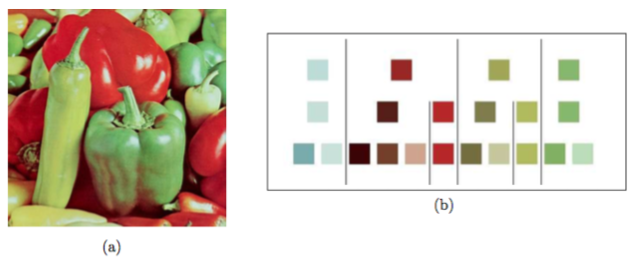
\includegraphics[width=0.48\textwidth]{img/peppers.png}
\caption{CPE Ergebnis von ACoPa. (a) Originalbild "Peppers" (b) Hierarchische Farbpalette. Die unterste Ebene zeigt die finalen Farben. (Quelle: \citep{acopa})}
\label{fig:peppers}
\end{figure}

\citet{acopa} kritisieren an den bisherigen Algorithmen, dass die Anzahl gesuchten Farben $n$ zuvor bekannt sein muss, dass die Ergebnisse abhängig von der Initialisierung sind und dass Farben kleiner Bilddetails im Sinne der Definition in Abschnitt \ref{sec:modellierung} nur unzureichend repräsentiert werden, wie im Paper experimentell nachgewiesen wird. Aus diesem Grund stellen sie den \textbf{Automatic Color Palette (ACoPa)} Algorithmus vor, welcher durch die Analyse von Spitzen des Histogramms im HSI Raums eine Farbpalette erstellt und dabei deren Größe selbstständig bestimmt. Der Algorithmus ermittelt dabei zunächst die grundlegenden Farbtöne (Hue) des Bildes und schlüsselt diese daraufhin sukzessive nach deren Sättigungen (Saturation) und Schattierungen (Intensity) auf. Abbildung \ref{fig:peppers} veranschaulicht exemplarisch die hierarchische Arbeitsweise, bei der in jeder Ebene zusätzliche Sättigungen und Schattierungen der enthaltenen roten und grünen Farbtöne gebildet werden.

\subsection*{Zusammenfassung und Wahl des Algorithmus zur CPE}

Der Algorithmus zur CPE soll eine Obermenge $C_s$ von Farben bilden, aus welcher im einem nachfolgenden Schritt eine Teilmenge von Farben $C$ entsprechend ihrer Eignung für bestimmte Oberflächenelemente ausgewählt werden. Analog dazu werden Farbpaletten in Styleguides als Obermenge von Farben beschrieben, aus welcher der Designer eine Untermenge von Farben für die konkrete Oberfläche auswählt. Bestimmte Styleguides erweitern dabei das Farbpalettenkonzept um Color Swatches, bei welchen Farbtöne in zusätzliche Schattierungen aufgefächert werden. Dadurch hat der der Designer eine größere Flexibilität beim Einsatz der Farbpalette.

Aus diesen Gründen wird der ACoPa Algorithmus von \citet{acopa} zur CPE gewählt. Da er Farbwerte automatisiert in verschiedenen Sättigungen und Schattierungen ermittelt, imitiert er die Farbdefinition in Form von Color Swatches in Styleguides. Durch seine parameterfreie Arbeitsweise ermittelt er selbstständig die Anzahl repräsentativer Farben im Bild. Dadurch wird automatisch die erforderliche Obermenge zur Bildung der finalen Farbpalette bereitgestellt, wenn das Bild ausreichend viele Farben enthält. Das erzwingen eines großen Farbpalette mit anderen Clusteringverfahren, z.B. über einen pauschal großen K Parameter bei K-Means, führt hingegen unter Umständen zu einer Partitionierung des Farbraums, die nicht der Clusterstruktur des Histogramms entspricht.

\section{ACoPa}

Im Folgenden wird die grundlegende Arbeitsweise des ACoPa Algorithmus nach \citet{acopa} vorgestellt. Dabei werden die Herausforderungen, die bei der Implementierung aufgetreten sind, besprochen. Abschließend werden exemplarisch Anwendungsergebnisse präsentiert.

\subsection{Konvertierung in den HSI-Raum}

\begin{figure*}
\centering
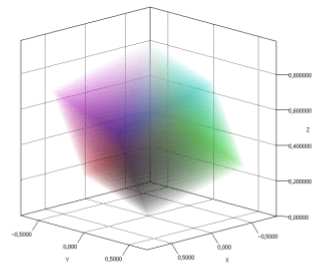
\includegraphics[width=1\textwidth]{img/hsi_conversion.png}
\caption{Gegenüberstellung von RGB zu HSI-Umrechungsergebnisse. (a.) Referenz-HSI Raum. (b.) Umrechnung nach \citep{acopa}. (c.) Umrechnung nach \citep{colorimage}.}
\label{fig:hsi_conversion}
\end{figure*}

Zunächst wird das Histogram in den HSI Farbraum $\{(h, s, i) \ | \ 0 \leq h < 360 \wedge 0 \leq s, i \leq 1\}$ übertragen. Die Intensität eines Farbtons wird dabei in Polarkoordinaten via $h$ und $s$ angegeben, während die maximal mögliche Sättigung wiederum von der Intensität $i$ abhängt. Zur Konvertierung vom RGB in HSI Raum wurden verschiedene Umrechnungsvorschriften erprobt. Die Umrechnung gemäß der ACoPa-Autoren lautet:

\begin{equation}
\begin{split}
I = \frac{R+G+B}{3} \\
S = \sqrt{(R-I)^2 + (G-I)^2 + (B-I)^2} \\  
H = \arccos{(\frac{(G-I)-(B-I)}{S\sqrt{2}})}
\end{split}
\label{eq:hsi_acopa}
\end{equation}

Die Umrechnung gemäß eines Lehrbuchs für Farbbild-Verarbeitung \citep{colorimage} lautet hingegen:

\begin{equation}
\begin{split}
I = \frac{R+G+B}{3} \\
S = 1 - \frac{\min{(R, G, B)}}{I} \\ 
H = \arccos{(\frac{\frac{1}{2}((R-G)+(R-B))}{\sqrt{(R-G)^2+(R-B)(G-B))}})}
\end{split}
\label{eq:hsi_colorimage}
\end{equation}

Abbildung \ref{fig:hsi_conversion} stellt die Umrechnungsergebnisse dem Referenz HSI Raum (R) gegenüber. Keine der Umrechnungsvorschriften führt zu einem Doppelkegel. Weder Formel \ref{eq:hsi_acopa} noch Formel \ref{eq:hsi_colorimage} projiziert die Farben mit 100\% Sättigung ($s = 1$) in eine Ebene. Formel \ref{eq:hsi_acopa} führt lediglich zu einer Drehung und Stauchung des RGB-Würfels, Formel \ref{eq:hsi_colorimage} führt zu einem nach unten geöffneten Kegel. Da schlussendlich keine Formel gefunden werden konnte, die zu einem korrekten Doppelkegel führt, wurde die Berechnung mit Formel \ref{eq:hsi_acopa} fortgeführt.

\subsection{Histogramm-Segmentierung}

Die Samples des Ausgangsbildes werden entlang der Hue-Werte sortiert. Das 1-dimensionale Hue-Histogram $h=(h_i)_{i = 1 \ldots b}$ mit b-Bins wird gebildet. Gesucht wird nun eine Sequenz $s = (s_i)_{i = 1 \ldots k}$ mit $1 = s_0 < s_1 < \ldots < s_k = b$, welche eine Segmentierung des Histograms darstellt. Das Intervall $[{s_i}, s_{i+1}]$ wird als Segment bezeichnet. Ziel ist, dass das Histogramm in den Bereichen $[h_{s_i}, \ldots,  h_{s_{i+1}}]$, eine \glqq annähernd unimodale Verteilung aufweist\grqq \citep{acopa}. Abbildung \ref{fig:unimodal} zeigt das Prinzip an verschiedenen Beispielen.

\begin{figure}[h]
\centering
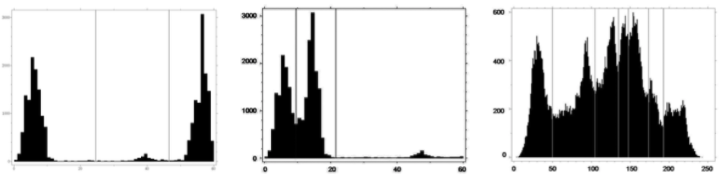
\includegraphics[width=0.48\textwidth]{img/unimodal.png}
\caption{Beispiele der Segmentierung eines Histograms in unimodale Abschnitte. (Quelle: \citep{acopa})}
\label{fig:unimodal}
\end{figure}

Das Histogramm ist offensichtlich in jedem Segment unimodal, wenn $s$ mit den Minima des Histograms initialisiert wird. Es wird nun versucht, Elemente aus $s$ zu entfernen, indem für $\forall i = 1 .. k$ überprüft wird, ob $h$ im Intervall $[h_{s_{i-1}}, \ldots,  h_{s_{i+1}}]$ die \glqq unimodale Hypothese\grqq  erfüllt. Anschaulich bedeutet das die Verschmelzung benachbarter Segmente, so dass das neu entstandene Segment nach wie vor \glqq annähernd unimodal ist\grqq. Hierfür stellen die Autoren in einer separaten Veröffentlichung \citep{ftc} einen parameterfreien statistischen Test vor, der $h$ im betrachteten Intervall mit einem Referenz-Histogramm $h^r$ vergleicht. $h^r$ ist in $[h^r_{s_{i-1}}, \ldots,  h^r_{s_{i+1}}]$ zunächst streng monoton wachsend und danach streng monoton fallend und damit in jedem Fall unimodal. Das Referenz-Histogramm wird aus dem Original-Histogramm $h$ durch Anwendung des Grenander-Operators gebildet. Die komplexen Details hierzu sind \citep{acopa, ftc} zu entnehmen. Da der parameterfreie Test verhältnismäßig aufwändig ist, wird in der eigenen Implementierung auf einen simplen T-Test zurückgegriffen. Dieser liefert ebenfalls befriedigende Ergebnisse, ist aber abhängig vom gewählten Signifikanzniveau.

Das Verfahren zur Histogramm-Segmentierung wird in \citep{ftc} als \textbf{Fine-to-Coarse (FTC) Segmentation Algorithm} zusammengefasst. Zunächst wird $s$ mit allen Minima des Histogramms initialisiert. Daraufhin werden so lange benachbarte Segmente durch Überprüfung der unimodalen Hypothese verschmolzen, bis keine Verschmelzung mehr möglich ist. Die Repräsentanten eines Segments werden durch Mittelung der Samples gebildet, die zum jeweiligen Segment gehören. Abbildung \ref{fig:h_segmentation} zeigt dies an einem Beispiel.

\begin{figure}[h]
\centering
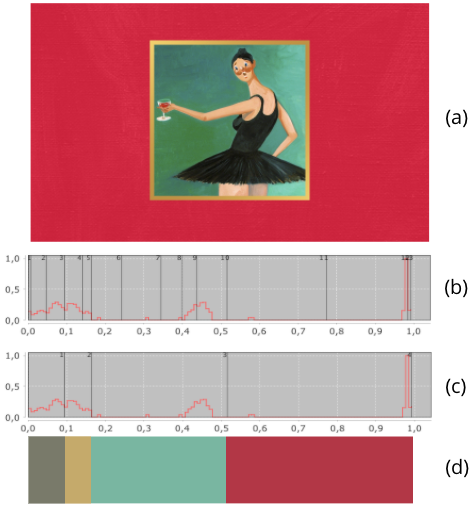
\includegraphics[width=0.48\textwidth]{img/h_segmentation.png}
\caption{Beispiel für eine Segmentierung des Hue-Histogramms. (a) Ausgangsbild, ein Albumcover  von Kanye West. (b) Hue-Histogram (normalisiert), mit allen Minima als initiale Segmentierung. (c) Segmentierung nach Anwendung des FTC Algorithmus. (d) Farbmittelpunkte entsprechend der Samples der jeweiligen Segmente.}
\label{fig:h_segmentation}
\end{figure}

\subsection{Bildung der hierarchischen Farbpalette}

Der ACoPa Algorithmus besteht aus einer hierarchischen Anwendung der Histogram-Segmentierung. Dabei wird zuerst der $h$-, danach der $s$- und abschließend der $i$- Kanal segmentiert. Dabei werden in jedem Schritt die Samples der entstandenen Segmente separiert und die Histogramme der nächsten Ebene getrennt berechnet. Das Ergebnis ist eine hierarchische Farbpalette. Abbildung \ref{fig:palette} zeigt dies am Beispiel der Covers aus Abbildung \ref{fig:h_segmentation}. Auf oberster Ebene (h) wurden die grundsätzlichen Farbtöne des Bildes identifiziert. Auf der zweiten Ebene werden die Farbtöne jeweils in unterschiedliche Sättigungen aufgeteilt, wenn nötig. Auf der dritten Ebene (i) werden von den Sättigungen zusätzlich Helligkeitsabstufungen gebildet.

Die letzte Ebene (i) bildet die Obermenge der Farben $C_s$ für die weitere Verarbeitung. \citet{acopa} empfehlen zusätzlich, die erhaltenen Farben als Startpunkte für den K-Means Algorithmus zu verwenden. Abbildung \ref{fig:palette} (b) zeigt, wie sich die Farben durch K-Means geändert haben. Es ist zu einem späteren Zeitpunkt zu entschieden, welche der beiden Paletten für die weitere Verarbeitung geeigneter ist.

\begin{figure}[h]
\centering
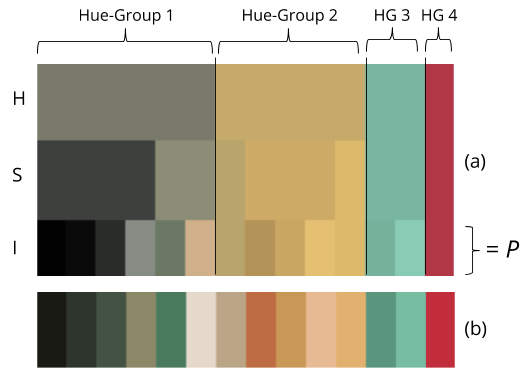
\includegraphics[width=0.48\textwidth]{img/palette.png}
\caption{(a) Hierarchische Farbpalette des Covers aus Abbildung \ref{fig:h_segmentation}. (b) Farbpalette nach Anwendung von K-Means.}
\label{fig:palette}
\end{figure}




\bibliographystyle{plainnat_ger}
\footnotesize{\bibliography{references}}

\end{document}
